\documentclass[a4paper,12pt,twoside]{article}

\usepackage{graphicx}
\usepackage{polski}
\usepackage[utf8]{inputenc}
\usepackage{indentfirst}
\usepackage{float}
\usepackage{listings}
\usepackage[scaled]{helvet}
\usepackage{fancyhdr}
\usepackage{pdfpages}
\usepackage[labelsep=period]{caption}
\usepackage{amsmath}
\usepackage{hyphenat}
\usepackage[shortlabels]{enumitem}
\usepackage[titletoc, title]{appendix}
\usepackage{chngcntr}

\renewcommand\familydefault{\sfdefault} 
\usepackage[T1]{fontenc}


\title{Praca inżynierska}
\author{Tomasz Kogowski}

\pagestyle{fancy}
\fancyhf{}
 
\renewcommand{\headrulewidth}{0pt}
\renewcommand{\baselinestretch}{1.15} 

\newcommand{\source}[1]{\caption*{\emph{\footnotesize Źródło elementów graficznych: {#1}.}} }
\fancyfoot[LO,RE]{\thepage}\pagestyle{fancy}

\begin{document}

\includepdf[pages=1]{pierwsza_strona/pierwsza_strona.pdf}
\pagenumbering{arabic}
\newpage 
\section*{Streszczenie}
\newpage 
\section*{Abstract}

\newpage
%\section*{Oświadczenie o autorstwie pracy}
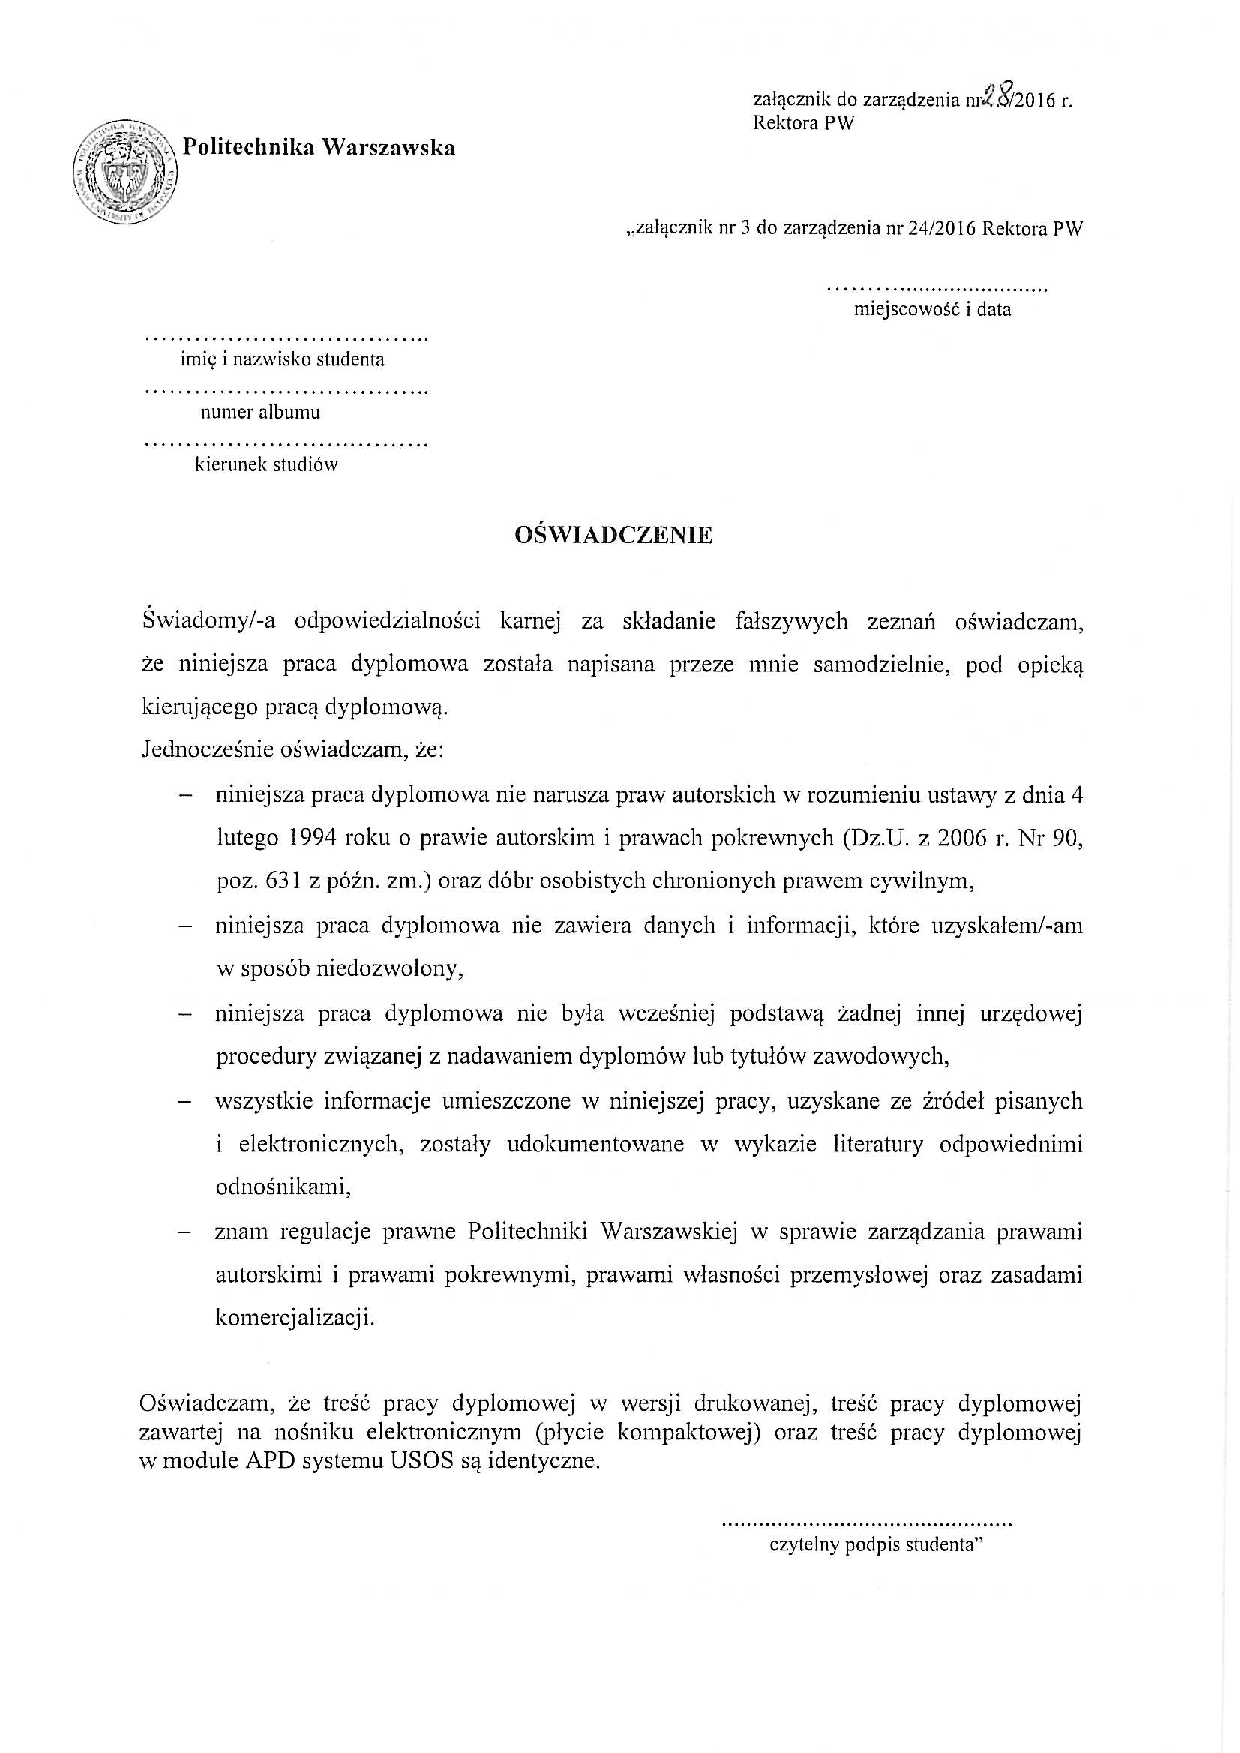
\includepdf[pages=1]{obrazy/oswiadczenie.pdf}
\newpage
\tableofcontents
 
\newpage
\section{Wstęp}  
\newpage
\section{Wymagania funkcjonalne i niefunkcjonalne}  
\newpage
\section{Systemy podobne}  
\paragraph{skupić się na tym iż systemy nie pozwalają na personalizacje interfejsu dla użytkownika}
\newpage
\section{Wybór technologi}
\subsection{Język programowania Scala}
\subsection{System zarządzania bazą danych PostgreSQL}  
\subsection{Platforma programistyczna Play}
\newpage
\section{Przypadki użycia}

\subsection{Autoryzacja}
\subsubsection{Role}
\subsubsection{Rejestracja użytkownika}
\subsubsection{Logowanie użytkownika}

\subsection{Przeglądanie danych z sekwencjownowania DNA}
\subsubsection{Widok listy dostępnych próbek}
\subsubsection{Ekran dostępnych genomów}
\subsubsection{Filtrowanie danych}

\subsection{Panel administratora}
\subsubsection{Zarządzanie filtrami}
\subsubsection{Zarządzanie rolami użytkowników}
\subsubsection{Zarządzanie widocznością próbek dla użytkowników}
\newpage
\section{Schemat bazy danych}
\newpage
\section{Opis implementacji}  
\newpage
\section{Bezpieczeństwo aplikacji}  
\subsection{Niebezpieczeństwa}
\subsection{Wykorzystanie protokołu https}

\subsection{}

\newpage
\section{Testy oraz wydajność}  
\newpage
\section{Wnioski i podsumowania}  

\addcontentsline{toc}{section}{Literatura}
\newpage
\begin{thebibliography}{99}
\end{thebibliography}

\newpage
\section*{Wykaz rysunków i tabel} 
\end{document}